% Dokumenteneinrichtung                                                         %
    \documentclass[                                                             %┐
        12pt,                                                                   %├╴Dokumentenklasse mit Standardschriftgröße
        twoside                                                                 %│ (`twosided` für doppelseitige Dokumente auskommentieren)
    ]{scrartcl}                                                                 %┘
    \usepackage[english]{babel}                                                 %─╴Sprachunterstützung
    \usepackage{hyperref}  											            %─╴Links & Formulare im PDF
% Kodierung                                                                     %
    \usepackage[utf8]{inputenc}                                                 %─╴Dateikodierung (benutze `[latin1]` statt [utf8], wenn Editor kein UTF-8 unterstützt)
    \usepackage[T1]{fontenc}                                                    %─╴Ausgabekodierung
% PDF-Metainformationen                                                         %
    \hypersetup{                                                                %┐
        pdfauthor={Berg, D. \& Reimer, J. H.},                     %├╴PDF-Metainformationen
        pdftitle={Analyzing the Million Song Dataset}                           %│
    }                                                                           %┘
% Seitenlayout                                                                  %
    \usepackage[                                                                %┐
        a4paper,                                                                %├╴Seitengröße und -abstände (`inner`=`left` in einseitigen Dokumenten)
        inner=3cm,                                                              %│
        outer=3cm,                                                              %│
        top=3.55cm,                                                             %│
        bottom=3cm,                                                             %│
        head=0.55cm,                                                            %│
    ]{geometry}                                                                 %┘
% Schriftarten (bitte entsprechend auskommentieren)                             %
    % \usepackage{lmodern}                                                      %─╴Latin Modern (Fließtext, moderne Alternative zu "Computer Modern")
    \usepackage[default,regular]{sourceserifpro}                              %─╴Source Serif Pro (Fließtext, unterstützt keinen kursiven Text)
    % \usepackage{heuristica}\renewcommand*{\oldstylenums}[1]{\textosf{#1}}       %─╴Heuristica (Fließtext)
    \usepackage{sourcesanspro}                                                  %─╴Source Sans Pro (Überschriften)
    \usepackage{eulervm}                                                        %─╴Euler Maths (Mathe-Modus)
    \usepackage[ttdefault]{sourcecodepro}                                       %─╴Source Code Pro (Code)
% Schriftdarstellung                                                            %
    \linespread{1.25}                                                           %─╴Zeilenabstand
    % \setlength{\parindent}{0pt}                                               %─╴Auskommentieren, um Einrückung der Absätze zu deaktivieren
% Schriftformatierung                                                           %
    \newcommand{\email}[1]{\href{mailto:#1}{\nolinkurl{#1}}}                                %─╴Fett
% Titel                                                                         %
    \title{Analyzing the Million Song Dataset}                                  %─╴Titel
    %\subtitle{}                                                                %─╴Untertitel
    \author{%                                                                   %─╴Autor des Dokuments
        Berg, Dmitrij \\
        {\small\email{dmitrij.berg@student.uni-halle.de}}
        \and
        Reimer, Jan Heinrich \\
        {\small\email{jan.reimer@student.uni-halle.de}}
    }
    \date{\today}                                                               %─╴Datum des Dokuments
    \setkomafont{title}{\sffamily\bfseries\Huge\centering}                      %─╴Titel-Schriftart
    \setkomafont{subtitle}{\sffamily\fontseries{sb}\Large\centering}            %─╴Untertitel-Schriftart
    \setkomafont{author}{\sffamily\large\centering}                             %─╴Datums-Schriftart
    \setkomafont{date}{\sffamily\large\centering}                               %─╴Autoren-Schriftart
% Kopf-/Fußzeile                                                                %
    \usepackage[headsepline,singlespacing=true]{scrlayer-scrpage}               %┐
    \pagestyle{scrheadings}                                                     %┴╴Kopf- und Fußzeilen-Paket
    \clearpairofpagestyles                                                      %─╴Inhalt der Kopf- und Fußzeile zurücksetzen
    \setkomafont{pageheadfoot}{\sffamily}                                       %─╴Kopfzeilen-Schriftart
    \setkomafont{pagination}{\sffamily}                                         %─╴Fußzeilenschriftart-Schriftart
    \ohead{\pagemark}                                                           %─╴Kopfzeile außen
% Mathematik                                                                    %
    \usepackage{amssymb}                                                        %┐
    \usepackage{amstext}                                                        %├╴Mathematik-Pakete
    \usepackage{amsmath}                                                        %┘
% Grafik                                                                        %
    \usepackage{tabu}                                                           %─╴Tabeles with variable-width columns
    \usepackage{longtable}                                                      %─╴Tabeles over multiple pages
    \usepackage{booktabs}                                                       %─╴Better horizontal table row seperators
    \usepackage{graphicx}                                                       %─╴Grafiken und PDFs einfügen
    \usepackage{color}                                                          %─╴Text farbig darstellen
    \usepackage{rotating}                                                       %─╴Elemente rotieren
% Literaturverzeichnis (siehe `*.bib`-Datei für Quellenangaben)                 %
    \usepackage[backend=biber,style=authoryear,sortcites]{biblatex}
    \addbibresource{\jobname.bib}
    % \renewcommand{\bibsection}{\part*{\bibname}}                                %─╴Formatierung der Literaturverzeichnis-Überschrift
% Citation                                                                      %
    \usepackage{csquotes}                                                       %─╴Citation package
% Glossaries                                                                    %
    \usepackage[acronym]{glossaries}                                            %─╴Glossaries package
    \newacronym{msd}{MSD}{The Million Song Dataset}
    \newacronym{mxm}{MXM}{\emph{musiXmatch} lyrics dataset}
    \newacronym{ttg}{TTG}{\emph{tagtraum} genre annotation dataset}
    \newacronym{tsv}{TSV}{Tab-separated values}
    \newacronym{mir}{MIR}{Music Information Retrieval}
    \makeglossaries                                                             %─╴Parse glossaries
% Anhang                                                                        %
    \usepackage[toc]{appendix}                                                  %─╴Anhang im Inhaltsverzeichnis
% Dokumentenspezifische Pakete und Konfiguration (Hier können Pakete            %
% eingebunden werden, die nur in einem Speziellen Dokument benötigt werden.)    %
\usepackage{caption}
\usepackage{subfig}\captionsetup{lofdepth=2}
\usepackage{multirow}
\usepackage{tikz}
\usepackage{pgfplots}
% Dokument                                                                      %
\begin{document}                                                                %
%%%%%%%%%%%%%%%%%%%%%%%%%%%%%%%%%%%%%%%%%%%%%%%%%%%%%%%%%%%%%%%%%%%%%%%%%%%%%%%%%
%% Title page                                                                  %%
%%%%%%%%%%%%%%%%%%%%%%%%%%%%%%%%%%%%%%%%%%%%%%%%%%%%%%%%%%%%%%%%%%%%%%%%%%%%%%%%%
\begin{titlepage}%
    \begin{center}
        
\includegraphics[width=0.5\linewidth]{logo-mlu}%
    \end{center}
    \vfill%
    \begin{minipage}{\linewidth}
        \vspace*{-5em}%
        \maketitle
        \vspace*{-3em}%
    \end{minipage}%
	\vfill%
    {%
        \small
        \noindent
        Martin-Luther-Universität Halle-Wittenberg \\
        Institute of Computer Science \\
        Big Data Analytics \\
        
        \noindent%
        \def\arraystretch{1.25}%
        \setlength{\tabcolsep}{0pt}%
        \begin{tabu} to \linewidth {>{\sffamily\bfseries} l @{\extracolsep{2em}} X}
        	Lecturer:             & Prof. Dr. Matthias Hagen          \\
        	Semester:             & Summer 2018              \\
        	Students:             & Dmitrij Berg, Jan Heinrich Reimer \\
        	Matriculation numbers: & 216226012, 216204166              \\
        	Version:              & 1.0.0                             \\
        	Date:                 & \today
        \end{tabu}
    }
	\clearpage
\end{titlepage}
%%%%%%%%%%%%%%%%%%%%%%%%%%%%%%%%%%%%%%%%%%%%%%%%%%%%%%%%%%%%%%%%%%%%%%%%%%%%%%%%%
%% Abstract                                                                    %%
%%%%%%%%%%%%%%%%%%%%%%%%%%%%%%%%%%%%%%%%%%%%%%%%%%%%%%%%%%%%%%%%%%%%%%%%%%%%%%%%%

% New York is the hotttessst town for music artists.
%%%%%%%%%%%%%%%%%%%%%%%%%%%%%%%%%%%%%%%%%%%%%%%%%%%%%%%%%%%%%%%%%%%%%%%%%%%%%%%%%
%% Statutory declaration                                                       %%
%%%%%%%%%%%%%%%%%%%%%%%%%%%%%%%%%%%%%%%%%%%%%%%%%%%%%%%%%%%%%%%%%%%%%%%%%%%%%%%%%
\section*{Statutory declaration}

The authors of this paper, 
\emph{Dmitrij Berg}, born on \emph{16.03.1998}, and  
\emph{Jan Heinrich Reimer}, born on \emph{25.01.1998}, 
declare that they have authored this thesis independently, 
that they have not used other than the declared sources/resources, 
and that they have explicitly marked all material which has been quoted 
either literally or by content from the used sources. \\

{%
    \vspace*{0.5cm}%
    \noindent%
    \setlength{\tabcolsep}{0pt}%
    \begin{tabu} to \textwidth {l @{\extracolsep{1.5cm}} X}
       	Halle (Saale), \today \hspace{0.5cm} &                            \\
       	\cmidrule{1-1} \cmidrule{2-2}
       	{\footnotesize Date}                 & {\footnotesize Signatures}
    \end{tabu}
}
\clearpage

%%%%%%%%%%%%%%%%%%%%%%%%%%%%%%%%%%%%%%%%%%%%%%%%%%%%%%%%%%%%%%%%%%%%%%%%%%%%%%%%%
%% Table of contents                                                           %%
%%%%%%%%%%%%%%%%%%%%%%%%%%%%%%%%%%%%%%%%%%%%%%%%%%%%%%%%%%%%%%%%%%%%%%%%%%%%%%%%%
\tableofcontents
\clearpage
%%%%%%%%%%%%%%%%%%%%%%%%%%%%%%%%%%%%%%%%%%%%%%%%%%%%%%%%%%%%%%%%%%%%%%%%%%%%%%%%%
%% Content                                                                     %%
%%%%%%%%%%%%%%%%%%%%%%%%%%%%%%%%%%%%%%%%%%%%%%%%%%%%%%%%%%%%%%%%%%%%%%%%%%%%%%%%%

\section{Introduction}

\subsection{Motivation}

Out of the many applications of big data analytics,
from news headlines to video streaming metrics 
to the human DNS,
the subject of \gls{mir} is probably one of the most interesting.

Everyone can easily identify with the relevance of the \gls{mir}
as music accompanies us in everyday life.
May it be learning an instrument or mixing music.
Even just listening to music 
leads to a natural personal interest 
to learn what features distinguish songs we like 
from those we don't like.

\section{Data}

\textquote{The \gls{msd} is a freely-available collection 
of audio features and meta data for a million contemporary 
popular music tracks.}\parencite{bertin2012million}
It contains songs dated from 1922 to 2010 
and was collected 2010 in an effort to make a dataset 
of close to commercial size
available to researchers \parencite[591]{bertin2011million}.

That comprehensive collection of titles, artists, publishing year etc. 
--- with direct connections to further datasets 
such as lyrics or genres --- seems to be the optimal data source 
for music-based investigation.

\subsection{Structure}

The dataset contains 1\,000\,000 track files. 
Each one is stored in the HDF5 format \parencite{hdfgroup2018hdf5} 
and consists of the fields as in \textcite{bertin2012field}.
Along structural information on the song's beats, sections etc. 
the \gls{msd} also provides song meta information fetched 
from The Echo Nest as described by \textcite[592]{bertin2011million}.

\subsection{Additional datasets}

One major advantage of the \gls{msd} is 
that it provides easy access to 
additional third party data sets.
Many projects already exist, 
that build upon the \gls{msd} 
and provide additional data.

\subsubsection{The musiXmatch lyrics dataset}

While songs lyrics seem to be the most relevant 
information source to interpret the artist's intentions and feelings
that data is generally rarely open to the public
and protected by copyright restrictions.

Musixmatch, formerly called musiXmatch, 
\textquote{is the world’s largest lyrics platform}\parencite{musixmatch2018about}.
According to \textcite{bertin2012musixmatch} the \gls{mxm} provides 
bag-of-words lyrics for 237,662 tracks of the \gls{msd}.
Specifically when performing summarizing/reducing tasks 
on a big dataset like the \gls{msd} that bag-of-words structure
turns out to be equally useful as the full lyrics.

\subsubsection{The tagtraum genre annotations dataset}

The \gls{msd} itself 
\textquote{does not contain readily accessible genre labels. 
Therefore, multiple attempts have been made
to add song-level genre annotations}\parencite[241]{schreiber2015improving}.
The \gls{ttg} for the Million Song Dataset
benefits from combining multiple data sources, 
namely the Last.fm dataset \parencite{bertin2012lastfm}, 
the Top-MAGD dataset \parencite{schindler2012facilitating}
and the beaTunes Genre Dataset \parencite[241]{schreiber2015improving} 
as described by \textcite[244]{schreiber2015tagtraum}, 
to provide a reasonable good accuracy.

\section{Technical implementation}

For the purpose of analyzing the \gls{msd} 
the Hadoop map-reduce framework \parencite{apache2018hadoop}, 
running on a single-node cluster 
on the Java Virtual Machine, was chosen.
It scales up to big datasets very well 
and is very flexible for doing different map-reduce tasks.
The mappers, reducers, data- and other classes 
were written in the Kotlin language \parencite{jetbrains2018kotlin}.

\subsection{HDF5 song file input format}

A custom Hadoop input format 
and a serializable \texttt{Song} data class 
had to be written to support parsing 
respectively storing the HDF5 song files 
in a format usable in Hadoop.
Moreover that \texttt{Song} class has the advantage 
of conveniently accessing the fields of the HDF5 files,
especially the arrays, in the Hadoop mappers and reducers
without having to access the HDF5 file directly.

\subsection{Heatmap generation}

For the purpose of creating the heatmaps 
in \autoref{fig:average-familiarity-by-artist-b} 
and \autoref{fig:average-song-hotttnesss-by-artist-b}
a flexible Kotlin program was written that could read in
the \gls{tsv} output by Hadoop and draw the heatmap 
on a predefined background.

\subsection{Challenges}

\subsubsection{HDF5 native library}

During setting up the Hadoop cluster,
including the HDF5 data input format,
internally accessing the native HDF5 library, 
turned out to be difficult.

As normally each Hadoop data node 
is running on a separate physical machine,
the mappers running on the data nodes can not
access files on the name node.
Thus one needs to configure 
the native library on each data node separately.
Writing custom wrappers around the Hadoop analyze tool 
and using Hadoop file system's shared cache 
it was possible to share the HDF5 native library
across the data nodes.

\subsubsection{Single-node cluster}

Setting up Hadoop to run on a single-node cluster 
of course is not the supposed usage 
of the Hadoop architecture.
Though, as there was no multi-node cluster 
available to the authors at the time of writing, 
this project was limited to a single-node cluster
running on a standard consumer laptop.

For each analyzed input file Hadoop creates a mapper. 
Although normally each mapper can process 
multiple splits (regions) of a file, 
the custom input format made for HDF5 songs 
doesn't support splits --- neither does 
the underlying HDF5 library. 
Consequently Hadoop would have 
to create 1\,000\,000 mappers (10\,000 for the subset) 
which of course overflows the RAM 
on most consumer hardware.
Therefore only parts of the subset --- 
the \texttt{B} sub-folder containing a total 
of 2380 song files --- were analyzed.

Speaking of hardware limitations, 
apart from memory usage the used scripts 
don't use up all system resources such as CPU.
HDD access rates seem to be the main speed-limiting factor
for the mappers themselves.

\section{Studies}

\subsection{What are the main topics of different genres?}

When hearing music of some specific genres one sometimes 
could get the impression that all songs are about the same topics,
mostly using the same keywords.
In the following two different approaches on interpreting 
raw word counts output by the Hadoop map-reduce tasks
are being discussed.

\subsubsection{Most common nouns}

To get a good understanding of what topics are relevant in a given set of words
a good estimation is to look at the nouns contained in the set.
\autoref{tab:most-common-nouns-by-genre} shows the most common English nouns 
for each genre's lyrics.
Based on that list \autoref{tab:most-common-nouns-by-genre-summarized} 
shows a summarized view of the three most commonly used words in song lyrics
for each genre. Here words separated by slashes~(/) occurred equally often.

\begin{table}
    \caption[The three most common stemmed English nouns per genre.]{%
        The three most common stemmed English nouns per genre, 
        without normalization,
        taken from \autoref{tab:most-common-nouns-by-genre}.
    }
    \label{tab:most-common-nouns-by-genre-summarized}
    \centering
    \begin{tabu} spread 0.9\linewidth {l l}
    	\toprule
    	Genre         & Most common words                 \\ \midrule
    	Blues         & alley, love/place/ride/road/train \\
    	Country       & babi, love, jingl                 \\
    	Electronic    & adventur, disgrac/ritual          \\
    	Folk          & heart/hope, citi                  \\
    	International & call/ride, countri/eye            \\
    	Jazz          & doctor, time, life/love           \\
    	Latin         & danc, time, faith                 \\
    	Pop / Rock    & love, time, way                   \\
    	Rap           & light/shit, music                 \\
    	Reggae        & road, pictur, man                 \\
    	R'n'B         & call, stori, babi                 \\ \bottomrule
    \end{tabu}
\end{table}

Interestingly some stereotypes could therefore be disproved 
while some others were confirmed by the data:
Love is a consistent topic across many of the examined genres, 
including Blues, Country, Folk (\textquote{heart}), 
Jazz, Pop/Rock and R'n'B (\textquote{babi}).
And this strongly conflicts the stereotype 
that Blues would be all about sadness,
that is also supported by the fact that 
travelling (\textquote{place}, \textquote{ride}, 
\textquote{road}, \textquote{train}) is 
another frequent topic in Blues music.
While other genres' topics are as expected,
like Latin music being about dancing (\textquote{danc}) 
and religion (\textquote{faith}) --- most of Latin America 
is Christian religious \parencite{pew2015global} --- or 
International music being about countries (\textquote{counti}) 
and communication (\textquote{call}),
some other genres are dominated by words one would not expect.
For instance, \autoref{tab:most-common-nouns-by-genre-summarized} shows 
that rituals (\textquote{ritual}) are a frequent topic 
in Electronic music.

\subsubsection{Word count normalization}\label{sec:word-count-normalization}

Just looking for nouns certainly is not sufficient enough 
for being able to determine the main topic as it excludes words 
that might have a far more relevant meaning as only the nouns,
like verbs or adjectives.
Also nouns that could likewise be verbs or adjectives 
are overweighted in the results.

However that is not a trivial task as filling words, foreign words, names
or punctuation clutter the word lists for each genre.
For instance the lyrics of Latin music contain a lot of Spanish words.

To counteract for that filling words, foreign words, names 
and punctuation were filtered out the list:

\begin{addmargin}{3em}\footnotesize
    \&, a, all, am, an, and, aqui, are, be, been, but, ca, con, could,
    de, dem, denk, do, e, el, ella, en, es, esta, estou, for, get, got,
    had, have, he, her, hey, i, ich, if, ihr, in, is, it, just, la, let,
    me, mi, michael, mil, muy, my, nicht, no, not, não, o, of, oh, on,
    por, que, s, se, será, she, sie, so, su, t, te, that, the, they,
    this, to, tu, un, und, was, we, whi, will, with, would, y, you, your
\end{addmargin}

After filtering these words genres were filtered out 
if they had no word left that occurred 30 times or more often:

\begin{addmargin}{3em}
    International, Latin, Jazz, Folk, Blues
\end{addmargin}

Note that the filtered words as well as the minimal word count required 
for the further interpretation were chosen somewhat randomly by the authors.
That said, changing these parameters may have a great effect on the results. 
Nonetheless this approach was considered good enough as there's not much 
algorithmic assistance available to adequately filter out filling words.

\subsubsection{Most common words}

After filtering \autoref{tab:most-common-words-by-genre} shows the 
most common English words for each genre's lyrics.
\autoref{tab:most-common-words-by-genre-summarized} summarizes
the three most commonly used words for each of these genres.
Again slashes~(/) denote words that occurred equally often.

\begin{table}
    \caption[The three most common stemmed English words per genre.]{%
        The three most common stemmed English nouns per genre, 
        after normalization,
        taken from \autoref{tab:most-common-words-by-genre}.
    }
    \label{tab:most-common-words-by-genre-summarized}
    \centering
    \begin{tabu} spread 0.9\linewidth {l l}
    	\toprule
    	Genre      & Most common words            \\ \midrule
    	Country    & babi, like, love             \\
    	Electronic & there, go, now               \\
    	Pop / Rock & know, never, love            \\
    	Rap        & die, like, up                \\
    	Reggae     & road, pictur, like/man/while \\
    	R'n'B      & call, feel, stori            \\ \bottomrule
    \end{tabu}
\end{table}

This view on the data shows a much more diverse result as verbs 
and presumably important words support the meaning of main topics
and especially interpreting it.

The topic of love in contrast to \autoref{tab:most-common-nouns-by-genre-summarized}
doesn't outweigh other equally important topics. 
Rather uncommon words like \textquote{disgrac} or \textquote{ritual} 
don't dominate lyrics of Electronic music anymore, 
instead \autoref{tab:most-common-words-by-genre-summarized} shows 
that in this genre things are not as important 
as activities (\textquote{go}, \textquote{now}).
In Pop/Rock music the word \textquote{never} comes to attention.
This may denote desires or unfulfilled dreams,
maybe related to \textquote{love}.
The most commonly used words in the genres of Country and R'n'B 
remain almost unchanged, main topics being 
feelings (\textquote{feel}, \textquote{like}) 
and love (\textquote{babi}, \textquote{love}, \textquote{call}).


\subsection{Where do the most familiar artists live?}

\begin{table}
    \centering
    \caption[Artists and locations with the highest average familiarity.]{%
        Artists and locations with the highest average familiarity.
        See \autoref{tab:artists-highest-average-familiarity-b}.
    }
    \label{tab:artists-highest-average-familiarity-b-locations}
    \begin{tabu} to \linewidth {r X r l}
    	\toprule
    	Rank & Artist name                  & Average familiarity & Location               \\ \midrule
    	  2. & Lil Wayne                    & 0.990               & New Orleans, LA, USA   \\
    	  3. & Britney Spears               & 0.947               & Los Angeles, CA, USA   \\
    	  4. & Avril Lavigne                & 0.942               & Belleville, ON, Canada \\
    	  7. & Alicia Keys                  & 0.934               & New York City, NY, USA \\
    	  8. & Muse                         & 0.929               & UK                     \\
    	  9. & Slipknot                     & 0.929               & Des Moines, IA, USA    \\
    	 16. & Taking Back Sunday           & 0.912               & Long Island, NY, USA   \\
    	 20. & Daddy Yankee / Bounty Killer & 0.909               & Puerto Rico            \\
    	 22. & Natasha Bedingfield          & 0.901               & London, UK             \\
    	 26. & The Smashing Pumpkins        & 0.888               & Chicago, IL, USA       \\
    	 27. & Killswitch Engage            & 0.888               & Boston, MA, USA        \\ \bottomrule
    \end{tabu}
\end{table}

In the analyzed subset there were 1719 artists 
with known familiarity, 
of which 639 have a location linked to their name
in the \gls{msd}.

An artist's familiarity score can be understood 
as the likelihood that a randomly selected person recognizes them. 
On the map an artist's location resembles their last known residence.

A lot of successful artists are known to travel around the globe 
in order to create their music, however assuming 
that most of an artist's impact on the music industry 
is bound to where they live, 
it would be interesting to see if there are regions of the world 
where exceptionally many artists with a high familiarity score pile up.

\begin{figure}
    \centering
    \caption[Artist's familiarity for selected regions.]{%
        Artist's familiarity for selected regions.
        See \autoref{fig:average-familiarity-by-artist-b}.
    }
    \label{fig:average-familiarity-by-artist-b-usa-uk}
    \subfloat[for the USA]{
        \label{fig:average-familiarity-by-artist-b-usa}
        \frame{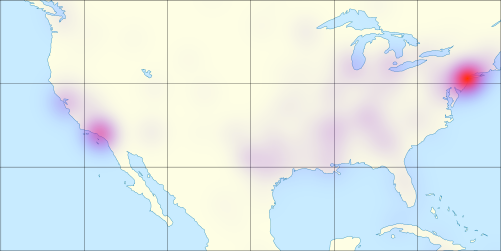
\includegraphics[width=0.6\linewidth]{../../results/average-familiarity-by-artist-B-cropped-usa}}
    }
    \hfill
    \subfloat[for the UK]{
        \label{fig:average-familiarity-by-artist-b-uk}
        \frame{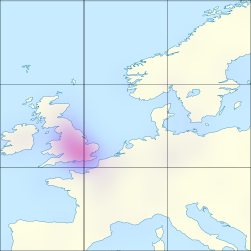
\includegraphics[width=0.3\linewidth]{../../results/average-familiarity-by-artist-B-cropped-uk}}
    }
\end{figure}

\autoref{fig:average-familiarity-by-artist-b} shows a world map on which 
for each coordinate the familiarity score of artists living there is
summed up using a lookup table that maps artist ID from the \gls{msd}
to their last known residence's coordinates.
While most of the world is empty, 
the USA and UK make up the most part of the familiarity score.
For better visibility \autoref{fig:average-familiarity-by-artist-b} has been cropped
to only show the USA (\autoref{fig:average-familiarity-by-artist-b-usa-uk}%
\subref{fig:average-familiarity-by-artist-b-usa}) 
respectively the UK (\autoref{fig:average-familiarity-by-artist-b-usa-uk}%
\subref{fig:average-familiarity-by-artist-b-uk}).

It turns out that big cities attract big personalities. 
New York City stands out as a glowing red spot, 
due to the vast number of instantly recognizable musicians 
originating in \textquote{the big apple}.%
\footnote{That nickname was frequently used by Jazz musicians in the 1930s.}
Artists like Jay-Z, Lady~Gaga, 50~Cent, Alicia~Keys 
and KISS --- just to name a few --- live there \parencite{ranker2018ny}.
As shown in \autoref{tab:artists-highest-average-familiarity-b}, 
Alicia Keys (7., 0.934) and 50~Cent (29., 0.883) are among the top 30, 
though only Alicia Keys' location is known in the \gls{msd}
(see \autoref{tab:artists-highest-average-familiarity-b-locations}).
And with a place that is known for attracting 
massive amounts of people by its tourist attractions 
and therefore is well known 
\parencite{nyc2018mayor}, 
the high familiarity in this region is quite obvious.

Los Angeles is another hot spot on the map. 
Artists like P!NK, Miley~Cyrus, Metallica, 
Guns'n'Roses (58., 0.844) or Red~Hot~Chili~Peppers (78., 0.834)
\parencite{ranker2018la}
might be essential to this bump in familiarity.
\autoref{tab:artists-highest-average-familiarity-b-locations} includes 
the Pop icon Britney~Spears (3., 0.947) as a familiar representative for Los Angeles, 
contributing to the clearly visible spot on the map 
(\autoref{fig:average-familiarity-by-artist-b-usa-uk}%
\subref{fig:average-familiarity-by-artist-b-usa}).

The city of Nashville is frequently called \textquote{music city USA}.
It achieved this nickname due to its vivid western 
and Country music scene \parencite{harper2013nashville}.
Naturally the \textquote{music city} should be home to popular artists.
Some of them like Kesha and Paramore are 
well known \parencite{ranker2018nashville}.
The comparatively low overall familiarity 
of Nashville can be explained 
by the steadily decreasing appeal of Country music worldwide.

Outside the US there is another colored spot on the world map, 
located in the UK, centered on London. 
That city features popular artists and bands 
like The~Rolling~Stones (102., 0.815), Led~Zeppelin (139., 0.787) 
and Amy~Winehouse \parencite{ranker2018london}.
\autoref{tab:artists-highest-average-familiarity-b-locations} includes 
Natasha~Bedingfield (22., 0.901) as a London-based very familiar musician.

\subsection{Where do the artists with the hotttessst songs live?}

\begin{table}
    \centering
    \caption[Artists and locations with the highest average song hotttnesss.]{%
        Artists and locations with the highest average song hotttnesss.
        Only the artists with known location with the highest 10 scores are shown.
        See \autoref{tab:artists-highest-average-song-hotttnesss-b}.
    }
    \label{tab:artists-highest-average-song-hotttnesss-b-locations}
    \begin{tabu} to \linewidth {r X r l}
    	\toprule
    	Rank & Artist name                 & Average song hotttnesss & Location                 \\ \midrule
    	  2. & The White Stripes           & 0.972                   & Detroit, MI, USA         \\
    	  4. & Nickelback                  & 0.910                   & Vancouver, BC, Canada    \\
    	  6. & Public Image Ltd            & 0.874                   & London, UK               \\
    	 10. & Britney Spears              & 0.840                   & Los Angeles, CA, USA     \\
    	 11. & Lighthouse Family           & 0.821                   & Newcastle upon Thyne, UK \\
    	 21. & The Radio Dept              & 0.788                   & Lund, Sweden             \\
    	 24. & Motograter                  & 0.771                   & Santa Barbara, CA, USA   \\
    	 26. & Lupe Fiasco                 & 0.764                   & Chicago, IL, USA         \\
    	 29. & Strata                      & 0.755                   & San José, CA, USA        \\
    	 30. & Arsonists Get All The Girls & 0.755                   & Santa Cruz, CA, USA      \\ \bottomrule
    \end{tabu}
\end{table}

A song's hotttnesss can be understood as the amount of 
online traffic, news headlines and listeners it recently 
(2010, when the \gls{msd} was created) generated.
Naturally it is likely that popular and well-recognized artists 
will generate awareness on their songs easier 
than newer, unknown artists as they already have more followers.
Their songs will create more headlines, 
have more listeners and result in a higher hotttnesss score.

A quick comparison of \autoref{fig:average-song-hotttnesss-by-artist-b} 
and \autoref{fig:average-familiarity-by-artist-b} shows little to no difference.
Presumably dominant spots on the world resemble \textquote{popularity-centers}
which unite 2010's most important songs.

\textcite{lamere2018hottt}, the Director of Developer Platform
at The Echo Nest, the company associated 
with creation of the \gls{msd} \parencite[591]{bertin2011million},
wrote about plotting each artist's familiarity
against their average song hotttnesss 
to detect upcoming popular artists, 
hence when their song's hotttnesss 
exceeds its author's familiarity.
The resulting plot shows that an artist's song hotttnesss 
is nearly proportional to their familiarity, with only few exceptions.
These become less likely to show up, the less data is shown.

Again the world map in \autoref{fig:average-song-hotttnesss-by-artist-b} has been cropped
to only show the USA (\autoref{fig:average-song-hotttnesss-by-artist-b-usa-uk}%
\subref{fig:average-song-hotttnesss-by-artist-b-usa}) 
respectively the UK (\autoref{fig:average-song-hotttnesss-by-artist-b-usa-uk}%
\subref{fig:average-song-hotttnesss-by-artist-b-uk}) for better visibility.

\begin{figure}
    \centering
    \caption[Artist's average song hotttnesss for selected regions.]{%
        Artist's average song hotttnesss for selected regions.
        Only the artists with known location with the highest 10 scores are shown.
        See \autoref{fig:average-song-hotttnesss-by-artist-b}.
    }
    \label{fig:average-song-hotttnesss-by-artist-b-usa-uk}
    \subfloat[for the USA]{
        \label{fig:average-song-hotttnesss-by-artist-b-usa}
        \frame{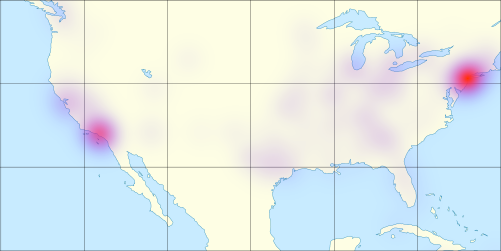
\includegraphics[width=0.6\linewidth]{../../results/average-song-hotttnesss-by-artist-B-cropped-usa}}
    }
    \hfill
    \subfloat[for the UK]{
        \label{fig:average-song-hotttnesss-by-artist-b-uk}
        \frame{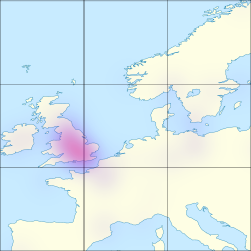
\includegraphics[width=0.3\linewidth]{../../results/average-song-hotttnesss-by-artist-B-cropped-uk}}
    }
\end{figure}

An example for a place that has less hottt songs than familiar artists 
is Nashville, Tennessee, USA. 
It doesn't show up in \autoref{fig:average-song-hotttnesss-by-artist-b-usa-uk}%
\subref{fig:average-song-hotttnesss-by-artist-b-usa}, 
meaning its popular musicians are losing listeners.

\section{Conclusions}

Analyzing just a small set of 2380 songs 
contained in the \texttt{B} sub-folder of 
the \gls{msd} subset, some results may not be as precise
because there's a greater chance of statistical outliers
to cause false interpretations.

\subsection{Analyzing the whole dataset}

A significant increase in size 
of the input data should slightly 
change the appearance of both 
\autoref{fig:average-familiarity-by-artist-b} 
and \autoref{fig:average-song-hotttnesss-by-artist-b} as well 
as improving meaningfulness of the lyrics analysis.
There would remain less \textquote{empty} space on the maps 
and potentially other regions of the world 
could form hot spots on the map.
The differences between familiarity and song hotttnesss
could also become more clear.
Less normalization would be required to get satisfactory
results when analyzing lyrics.

With the availability of a performant cluster 
analyzing the whole \gls{msd} would be possible 
without much modification of the scripts 
implemented for this thesis.
Given the \gls{msd}'s size of 1\,000\,000
and the analyzed subset's size of 2380 song files
a cluster of around 400 customer laptops would suffice
to answer the above questions for the whole \gls{msd}.
Of course that number of data nodes could be lowered
by using hardware with more memory capacity.

%%%%%%%%%%%%%%%%%%%%%%%%%%%%%%%%%%%%%%%%%%%%%%%%%%%%%%%%%%%%%%%%%%%%%%%%%%%%%%%%%
%% Postamble                                                                   %%
%%%%%%%%%%%%%%%%%%%%%%%%%%%%%%%%%%%%%%%%%%%%%%%%%%%%%%%%%%%%%%%%%%%%%%%%%%%%%%%%%
\clearpage
%%%%%%%%%%%%%%%%%%%%%%%%%%%%%%%%%%%%%%%%%%%%%%%%%%%%%%%%%%%%%%%%%%%%%%%%%%%%%%%%%
%% Glossaries                                                                  %%
%%%%%%%%%%%%%%%%%%%%%%%%%%%%%%%%%%%%%%%%%%%%%%%%%%%%%%%%%%%%%%%%%%%%%%%%%%%%%%%%%
%\printglossaries
%\clearpage
%%%%%%%%%%%%%%%%%%%%%%%%%%%%%%%%%%%%%%%%%%%%%%%%%%%%%%%%%%%%%%%%%%%%%%%%%%%%%%%%%
%% Acronyms ´                                                                  %%
%%%%%%%%%%%%%%%%%%%%%%%%%%%%%%%%%%%%%%%%%%%%%%%%%%%%%%%%%%%%%%%%%%%%%%%%%%%%%%%%%
\addcontentsline{toc}{section}{\acronymname}
\printacronyms
\clearpage
%%%%%%%%%%%%%%%%%%%%%%%%%%%%%%%%%%%%%%%%%%%%%%%%%%%%%%%%%%%%%%%%%%%%%%%%%%%%%%%%%
%% List of tables        ´                                                     %%
%%%%%%%%%%%%%%%%%%%%%%%%%%%%%%%%%%%%%%%%%%%%%%%%%%%%%%%%%%%%%%%%%%%%%%%%%%%%%%%%%
\addcontentsline{toc}{section}{\listtablename}
\listoftables
\clearpage
%%%%%%%%%%%%%%%%%%%%%%%%%%%%%%%%%%%%%%%%%%%%%%%%%%%%%%%%%%%%%%%%%%%%%%%%%%%%%%%%%
%% List of figures ´                                                           %%
%%%%%%%%%%%%%%%%%%%%%%%%%%%%%%%%%%%%%%%%%%%%%%%%%%%%%%%%%%%%%%%%%%%%%%%%%%%%%%%%%
\addcontentsline{toc}{section}{\listfigurename}
\listoffigures
\clearpage
%%%%%%%%%%%%%%%%%%%%%%%%%%%%%%%%%%%%%%%%%%%%%%%%%%%%%%%%%%%%%%%%%%%%%%%%%%%%%%%%%
%% Literaturverzeichnis                                                        %%
%%%%%%%%%%%%%%%%%%%%%%%%%%%%%%%%%%%%%%%%%%%%%%%%%%%%%%%%%%%%%%%%%%%%%%%%%%%%%%%%%
%\chapter*{\bibname}
\addcontentsline{toc}{section}{\refname}
\printbibliography
\clearpage
%%%%%%%%%%%%%%%%%%%%%%%%%%%%%%%%%%%%%%%%%%%%%%%%%%%%%%%%%%%%%%%%%%%%%%%%%%%%%%%%%
%% Anhang                                                                      %%
%%%%%%%%%%%%%%%%%%%%%%%%%%%%%%%%%%%%%%%%%%%%%%%%%%%%%%%%%%%%%%%%%%%%%%%%%%%%%%%%%
\appendix
\section{\appendixname}

%\sunbsection{Song file fields}\hfill
%
%{\scriptsize
%\begin{longtabu}{l l l}
%    \caption[Fields contained in the HDF5 file of a single song.]{
%        Fields contained in the HDF5 file of a single song. \parencite{bertin2012field}
%    }
%    \label{tab:song-field-list} \\ \toprule
%    Field name                                                                                                                             & Type                    & Description                                   \\ \midrule
%    \endfirsthead
%	\toprule
%	Field name                                                                                                                             & Type                    & Description                                   \\ \midrule
%	\endhead
%    \bottomrule
%    \endfoot
%    Analysis sample rate                                                                    & \texttt{Float}          & Sample rate of the audio used                 \\
%	Artist 7digitalid                                                                                                                      & \texttt{Int}            & ID from 7digital.com or -1                    \\
%	Artist familiarity                                                                                                                     & \texttt{Float}          & Algorithmic estimation                        \\
%	Artist hotttnesss                                                                                                                      & \texttt{Float}          & Algorithmic estimation                        \\
%	Artist id                                                                                                                              & \texttt{String}         & Echo Nest ID                                  \\
%	Artist latitude                                                                                                                        & \texttt{Float}          & Latitude                                      \\
%	Artist location                                                                                                                        & \texttt{String}         & Location name                                 \\
%	Artist longitude                                                                                                                       & \texttt{Float}          & Longitude                                     \\
%	Artist MusicBrainz ID                                                                                                                  & \texttt{String}         & ID from musicbrainz.org                       \\
%	Artist MusicBrainz tags                                                                                                                & \texttt{Array<String>}  & Tags from musicbrainz.org                     \\
%	Artist MusicBrainz tags count                                                                                                          & \texttt{Array<Int>}     & Tag counts for musicbrainz tags               \\
%	Artist name                                                                                                                            & \texttt{String}         & Artist name                                   \\
%	Artist Playme ID                                                                                                                       & \texttt{Int}            & ID from playme.com, or -1                     \\
%	Artist terms                                                                                                                           & \texttt{Array<String>}  & Echo Nest tags                                \\
%	Artist terms frequency                                                                                                                 & \texttt{Array<Float>}   & Echo Nest tags frequencies                    \\
%	Artist terms weight                                                                                                                    & \texttt{Array<Float>}   & Echo Nest tags weight                         \\
%	Audio md5                                                                                                                              & \texttt{String}         & Audio hash code                               \\
%	Bars confidence                                                                                                                        & \texttt{Array<Float>}   & Confidence measure                            \\
%	Bars start                                                                                                                             & \texttt{Array<Float>}   & Beginning of bars, usually on a beat          \\
%	Beats confidence                                                                                                                       & \texttt{Array<Float>}   & Confidence measure                            \\
%	Beats start                                                                                                                            & \texttt{Array<Float>}   & Result of beat tracking                       \\
%	Danceability                                                                                                                           & \texttt{Float}          & Algorithmic estimation                        \\
%	Duration                                                                                                                               & \texttt{Float}          & In seconds                                    \\
%	End of fade in                                                                                                                         & \texttt{Float}          & Seconds at the beginning of the song          \\
%	Energy                                                                                                                                 & \texttt{Float}          & Energy from listener point of view            \\
%	Key                                                                                                                                    & \texttt{Int}            & Key the song is in                            \\
%	Key confidence                                                                                                                         & \texttt{Float}          & Confidence measure                            \\
%	Loudness                                                                                                                               & \texttt{Float}          & Overall loudness in dB                        \\
%	Mode                                                                                                                                   & \texttt{Int}            & Major or minor                                \\
%	Mode confidence                                                                                                                        & \texttt{Float}          & Confidence measure                            \\
%	Release                                                                                                                                & \texttt{String}         & Album name                                    \\
%	Release 7digitalid                                                                                                                     & \texttt{Int}            & ID from 7digital.com or -1                    \\
%	Sections confidence                                                                                                                    & \texttt{Array<Float>}   & Confidence measure                            \\
%	Sections start                                                                                                                         & \texttt{Array<Float>}   & Largest grouping in a song, e.g. verse        \\
%	Segments confidence                                                                                                                    & \texttt{Array<Float>}   & Confidence measure                            \\
%	Segments loudness max                                                                                                                  & \texttt{Array<Float>}   & Max dB value                                  \\
%	Segments loudness max time                                                                                                             & \texttt{Array<Float>}   & Time of max dB value, i.e. end of attack      \\
%	Segments loudness max start                                                                                                            & \texttt{Array<Float>}   & dB value at onset                             \\
%	Segments pitches                                                                                                                       & \texttt{2dArray<Float>} & Chroma feature, one value per note            \\
%	Segments start                                                                                                                         & \texttt{Array<Float>}   & Musical events, ~ note onsets                 \\
%	Segments timbre                                                                                                                        & \texttt{2dArray<Float>} & Texture features (MFCC+PCA-like)              \\
%	Similar artists                                                                                                                        & \texttt{Array<String>}  & Echo Nest artist IDs (sim. algo. unpublished) \\
%	Song hotttnesss                                                                                                                        & \texttt{Float}          & Algorithmic estimation                        \\
%	Song id                                                                                                                                & \texttt{String}         & Echo Nest song ID                             \\
%	Start of fade out                                                                                                                      & \texttt{Float}          & Time in sec                                   \\
%	Tatums confidence                                                                                                                      & \texttt{Array<Float>}   & Confidence measure                            \\
%	Tatums start                                                                                                                           & \texttt{Array<Float>}   & Smallest rhythmic element                     \\
%	Tempo                                                                                                                                  & \texttt{Float}          & Estimated tempo in BPM                        \\
%	Time signature                                                                                                                         & \texttt{Int}            & Estimate of number of beats per bar, e.g. 4   \\
%	Time signature confidence                                                                                                              & \texttt{Float}          & Confidence measure                            \\
%	Title                                                                                                                                  & \texttt{String}         & Song title                                    \\
%	Track id                                                                                                                               & \texttt{String}         & Echo Nest track ID                            \\
%	Track 7digitalid                                                                                                                       & \texttt{Int}            & ID from 7digital.com or -1                    \\
%	Year                                                                                                                                   & \texttt{Int}            & Song release year from MusicBrainz or 0
%\end{longtabu}
%}

\subsection{Processed output data}


\subsubsection{Most common nouns per genre}

{\footnotesize
\begin{longtabu} to \linewidth {l X r r}
    \caption[Most common stemmed English nouns per genre, without normalization.]{%
        Most common stemmed English nouns per genre, without normalization.
        Words that could be both noun or verb are counted too.
        Only the highest three counts are shown.
    }
    \label{tab:most-common-nouns-by-genre} \\ \toprule
    Genre & Word & Count & Proportion \\ \midrule
    \endfirsthead
    \toprule
    Genre & Word & Count & Proportion \\ \midrule
    \endhead
    \bottomrule
    \endfoot
	Blues         & alley                                                            & 6      & 1,058\% \\*
	              & love, place, ride, road, train                                   & 4      & 0,705\% \\*
	              & babi, cruel, day, gin, people, salt, truth, wine, wound          & 3      & 0,529\% \\
	Country       & babi                                                             & 35     & 3,359\% \\*
	              & love                                                             & 17     & 0,845\% \\*
	              & jingl                                                            & 16     & 0,796\% \\
	Electronic    & adventur                                                         & 11     & 0,651\% \\*
	              & disgrac, ritual                                                  & 10     & 0,592\% \\*
	              & feet, look                                                       & 9      & 0,533\% \\
	Folk          & heart, hope                                                      & 7      & 0,552\% \\*
	              & citi                                                             & 6      & 0,474\% \\*
	              & eye, face, ride                                                  & 5      & 0,395\% \\
	International & call, ride                                                       & 5      & 1,285\% \\*
	              & countri, eye                                                     & 3      & 0,771\% \\*
	              & babe, daughter, day, father, fear, gentlemen, light, sheep, week & 2      & 0,514\% \\
	Jazz          & doctor                                                           & 5      & 1,160\% \\*
	              & time                                                             & 4      & 0,928\% \\*
	              & life, love                                                       & 2      & 0,464\% \\
	Latin         & danc                                                             & 11     & 0,596\% \\*
	              & time                                                             & 8      & 0,433\% \\*
	              & faith                                                            & 6      & 0,325\% \\
	Pop / Rock    & love                                                             & 162    & 0,621\% \\*
	              & time                                                             & 103    & 0,395\% \\*
	              & way                                                              & 88     & 0,338\% \\
	Rap           & light, shit                                                      & 25     & 0,387\% \\*
	              & music                                                            & 21     & 0,325\% \\*
	              & peopl                                                            & 17     & 0,263\% \\
	Reggae        & road                                                             & 44     & 3,839\% \\*
	              & pictur                                                           & 15     & 1,309\% \\*
	              & man                                                              & 11     & 0,960\% \\
	R'n'B         & call                                                             & 41     & 1,593\% \\*
	              & stori                                                            & 21     & 0,816\% \\*
	              & babi                                                             & 20     & 0,777\%
\end{longtabu}
}

\subsubsection{Most common words per genre}

{\footnotesize
\begin{longtabu}{l l r r}
    \caption[Most common stemmed English words per genre, after normalization.]{%
        Most common stemmed English words per genre, after normalization,
        explained in section \ref{sec:word-count-normalization}.
        Only the highest three counts are shown.
    }
    \label{tab:most-common-words-by-genre} \\ \toprule
    Genre & Word & Count & Proportion \\ \midrule
    \endfirsthead
    \toprule
    Genre & Word & Count & Proportion \\ \midrule
    \endhead
    \bottomrule
    \endfoot
	Country    & babi                       & 35  & 3,359\% \\*
	           & like                       & 24  & 2,303\% \\*
	           & love                       & 17  & 1,631\% \\
	Electronic & there                      & 30  & 3,421\% \\*
	           & go                         & 23  & 2,623\% \\*
	           & now                        & 17  & 1,938\% \\
	Pop / Rock & know                       & 176 & 1,353\% \\*
	           & never                      & 171 & 1,314\% \\*
	           & love                       & 162 & 1,245\% \\
	Rap        & die                        & 51  & 1,401\% \\*
	           & like                       & 35  & 0,962\% \\*
	           & up                         & 32  & 0,879\% \\
	Reggae     & road                       & 44  & 7,626\% \\*
	           & pictur                     & 15  & 2,600\% \\*
	           & like\slash man\slash while & 11  & 1,906\% \\
	R'n'B      & call                       & 41  & 3,071\% \\*
	           & feel                       & 26  & 1,948\% \\*
	           & stori                      & 21  & 1,573\%
\end{longtabu}
}

\subsubsection{Artists with the highest familiarity score}

{\footnotesize
\begin{longtabu}{r l r}
    \caption[Artists with the highest average familiarity.]{%
        Artists with the highest average familiarity, 
        rounded to three decimal places.
        Only the artists with the highest 30 scores are shown.
    }
    \label{tab:artists-highest-average-familiarity-b} \\ \toprule
    Rank & Artist name & Average familiarity \\ \midrule
    \endfirsthead
    \toprule
    Rank & Artist name & Average familiarity \\ \midrule
    \endhead
    \bottomrule
    \endfoot
	 1. & Akon / Kardinal Offishall  & 1.000 \\
	 2. & Lil Wayne                  & 0.990 \\
	 3. & Britney Spears             & 0.947 \\
	 4. & Avril Lavigne              & 0.942 \\
	 5. & Fall Out Boy               & 0.938 \\
	 6. & Mariah Carey               & 0.935 \\
	 7. & Alicia Keys                & 0.934 \\
	 8. & Muse                       & 0.929 \\
	 9. & Slipknot                   & 0.929 \\
	10. & The Game                   & 0.928 \\
	11. & Evanescence                & 0.921 \\
	12. & The Killers                & 0.918 \\
	13. & Big Daddy Rick             & 0.918 \\
	14. & Lily Allen                 & 0.916 \\
	15. & Madonna                    & 0.916 \\
	16. & Taking Back Sunday         & 0.912 \\
	17. & System of a Down           & 0.910 \\
	18. & 30 Seconds to Mars         & 0.909 \\
	19. & AFI                        & 0.909 \\
	20. & Daddy Yankee/Bounty Killer & 0.909 \\
	21. & Maroon 5                   & 0.905 \\
	22. & Natasha Bedingfield        & 0.901 \\
	23. & Radiohead                  & 0.900 \\
	24. & The Maine                  & 0.895 \\
	25. & New Found Glory            & 0.892 \\
	26. & The Smashing Pumpkins      & 0.888 \\
	27. & Killswitch Engage          & 0.888 \\
	28. & Beyoncé                    & 0.887 \\
	29. & 50 Cent                    & 0.883 \\
	30. & Janet Jackson              & 0.882
\end{longtabu}
}

\subsubsection{Artist's familiarity heatmap}

\begin{minipage}{\linewidth}
    \centering
    \frame{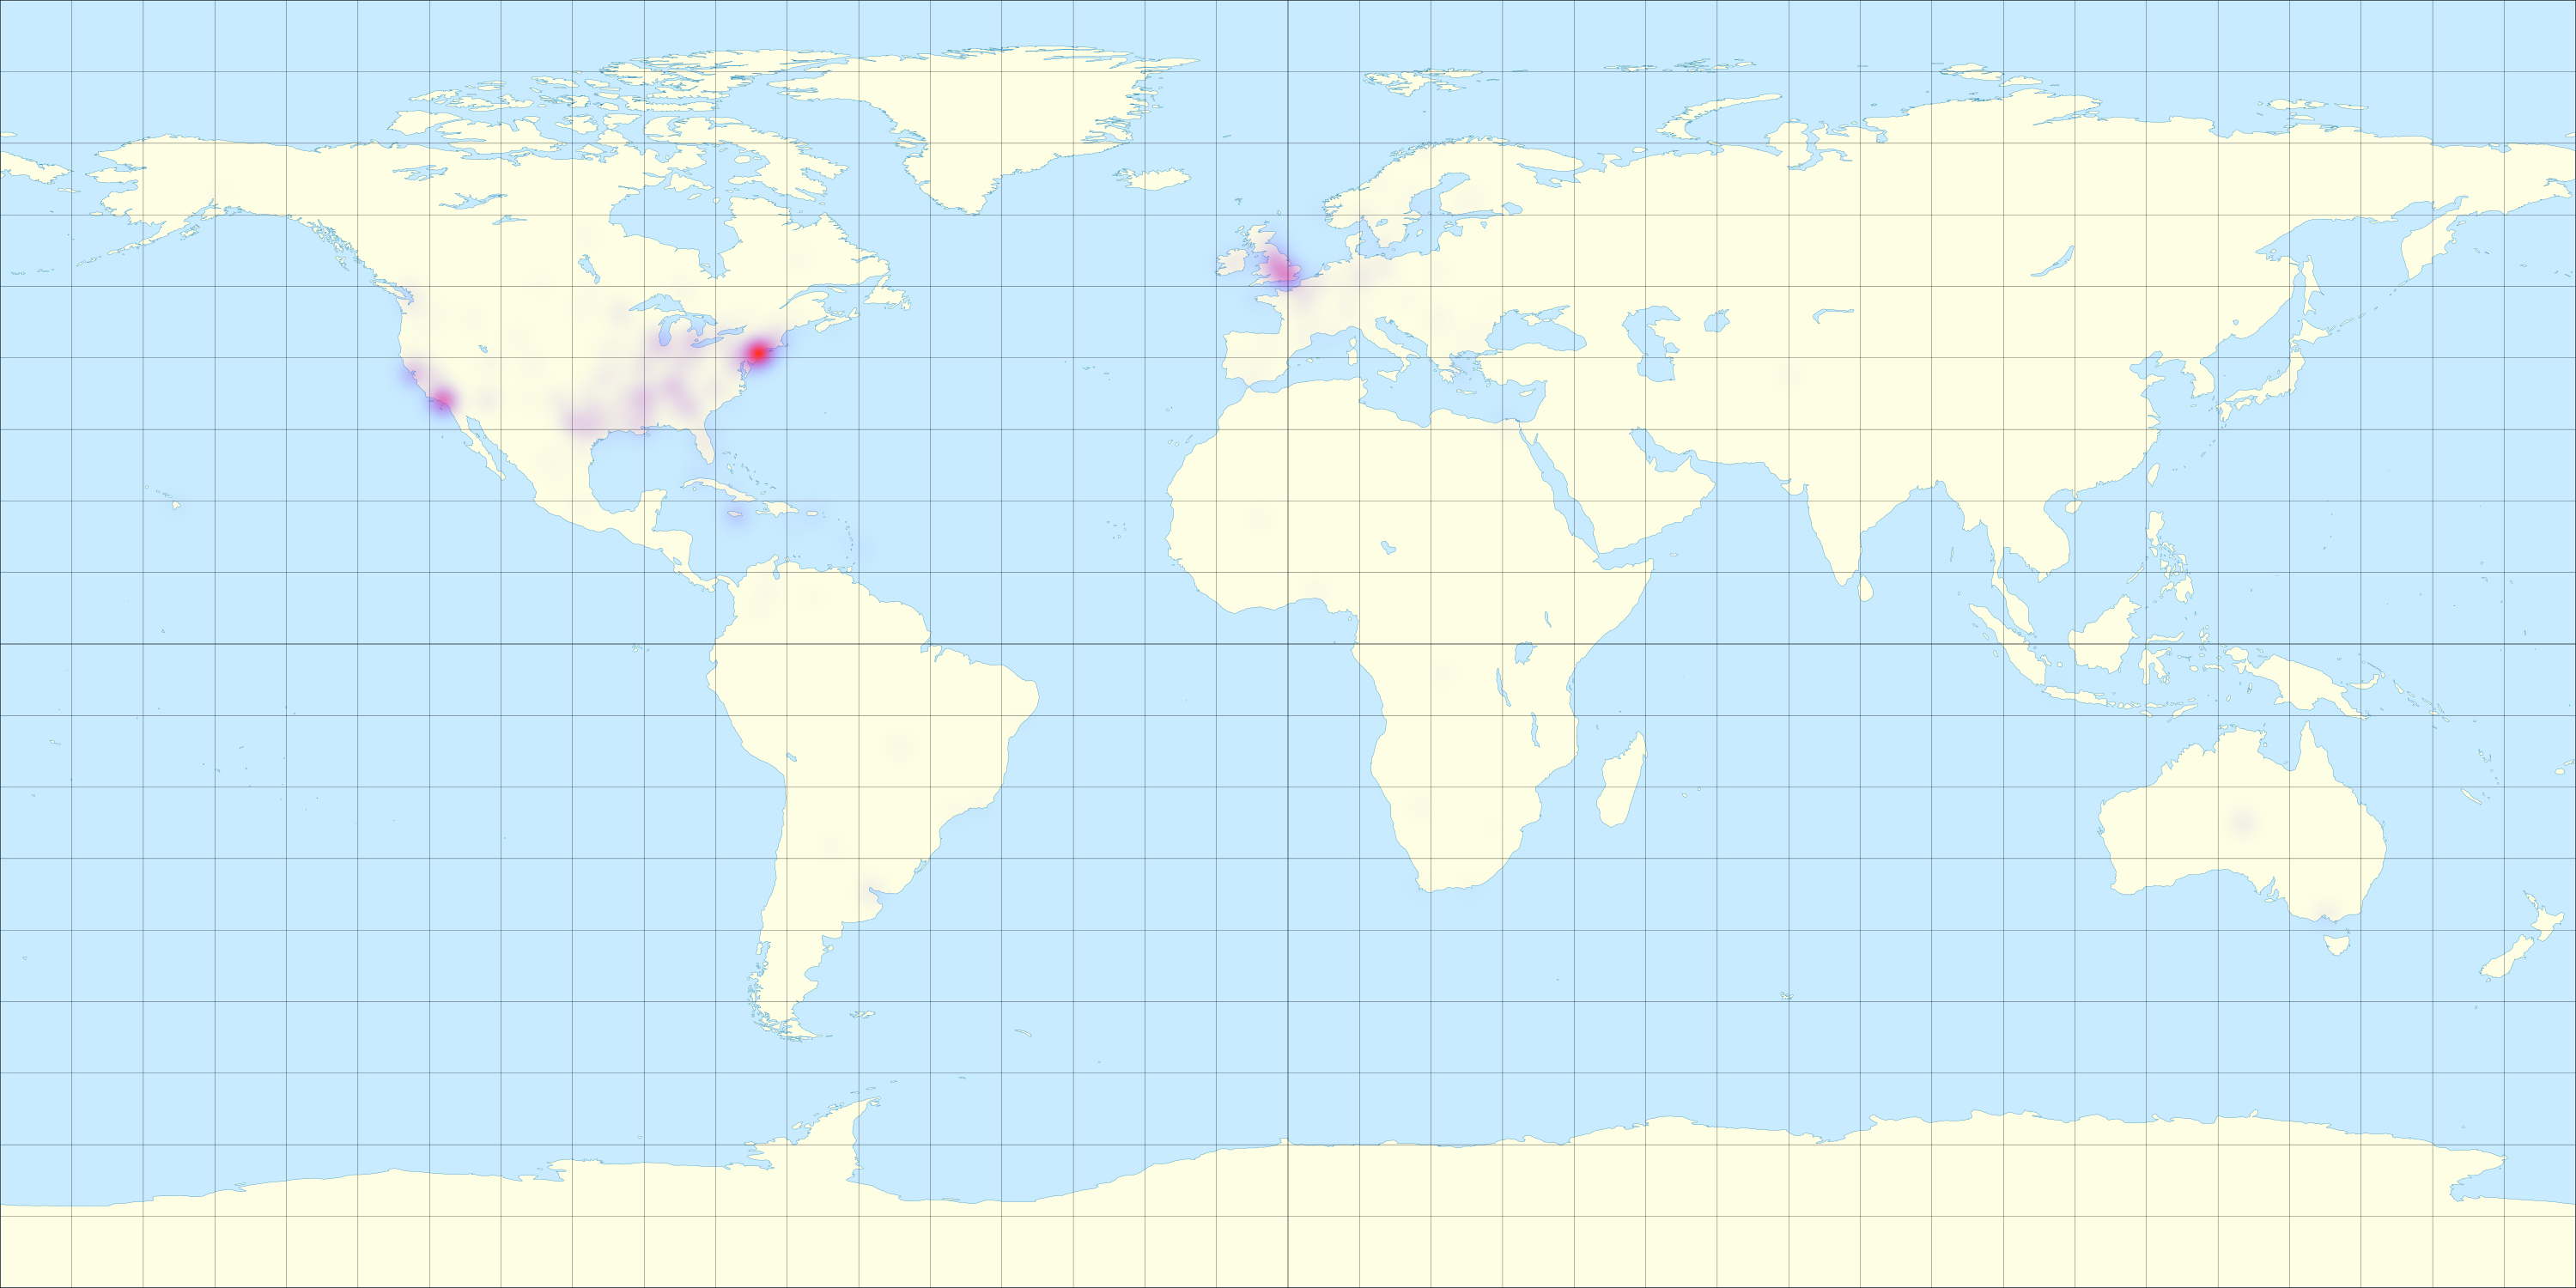
\includegraphics[width=\linewidth]{../../results/average-familiarity-by-artist-B}}
    \captionof{figure}[Artist's familiarity plotted on a map based on the artist's location.]{%
        Artist's familiarity plotted on a map based on the artist's location (if known).
        Adapted from \textcite{gaba2008tissot}.
    }
    \label{fig:average-familiarity-by-artist-b}
\end{minipage}

\subsubsection{Artists with the highest song hotttnesss score}

{\footnotesize
\begin{longtabu}{r l r}
    \caption[Artists with the highest average song hotttnesss.]{%
        Artists with the highest average song hotttnesss, 
        rounded to three decimal places.
        Only the artists with the highest 30 scores are shown.
    }
    \label{tab:artists-highest-average-song-hotttnesss-b} \\ \toprule
    Rank & Artist name & Average song hotttnesss \\ \midrule
    \endfirsthead
    \toprule
    Rank & Artist name & Average song hotttnesss \\ \midrule
    \endhead
    \bottomrule
    \endfoot
	 1. & Led Zeppelin                & 1.000 \\
	 2. & The White Stripes           & 0.972 \\
	 3. & The Mars Volta              & 0.929 \\
	 4. & Nickelback                  & 0.910 \\
	 5. & Thrice                      & 0.876 \\
	 6. & Public Image Ltd            & 0.874 \\
	 7. & Charlotte Gainsbourg        & 0.870 \\
	 8. & The Maine                   & 0.850 \\
	 9. & Temple of the Dog           & 0.849 \\
	10. & Britney Spears              & 0.840 \\
	11. & Lighthouse Family           & 0.821 \\
	12. & Porcupine Tree              & 0.821 \\
	13. & AFI                         & 0.814 \\
	14. & ATB                         & 0.811 \\
	15. & Spooky Tooth                & 0.807 \\
	16. & Salt-N-Pepa                 & 0.806 \\
	17. & Pink Floyd                  & 0.793 \\
	18. & System of a Down            & 0.792 \\
	19. & The Jeff Healey Band        & 0.789 \\
	20. & 30 Seconds to Mars          & 0.789 \\
	21. & The Radio Dept              & 0.788 \\
	22. & Xmilk                       & 0.783 \\
	23. & Ayo                         & 0.771 \\
	24. & Motograter                  & 0.771 \\
	25. & Cake                        & 0.764 \\
	26. & Lupe Fiasco                 & 0.764 \\
	27. & Van Halen                   & 0.760 \\
	28. & Chris Rea                   & 0.758 \\
	29. & Strata                      & 0.755 \\
	30. & Arsonists Get All The Girls & 0.755
\end{longtabu}
}

\subsubsection{Artist's song hotttnesss heatmap}

\begin{minipage}{\linewidth}
    \centering
    \frame{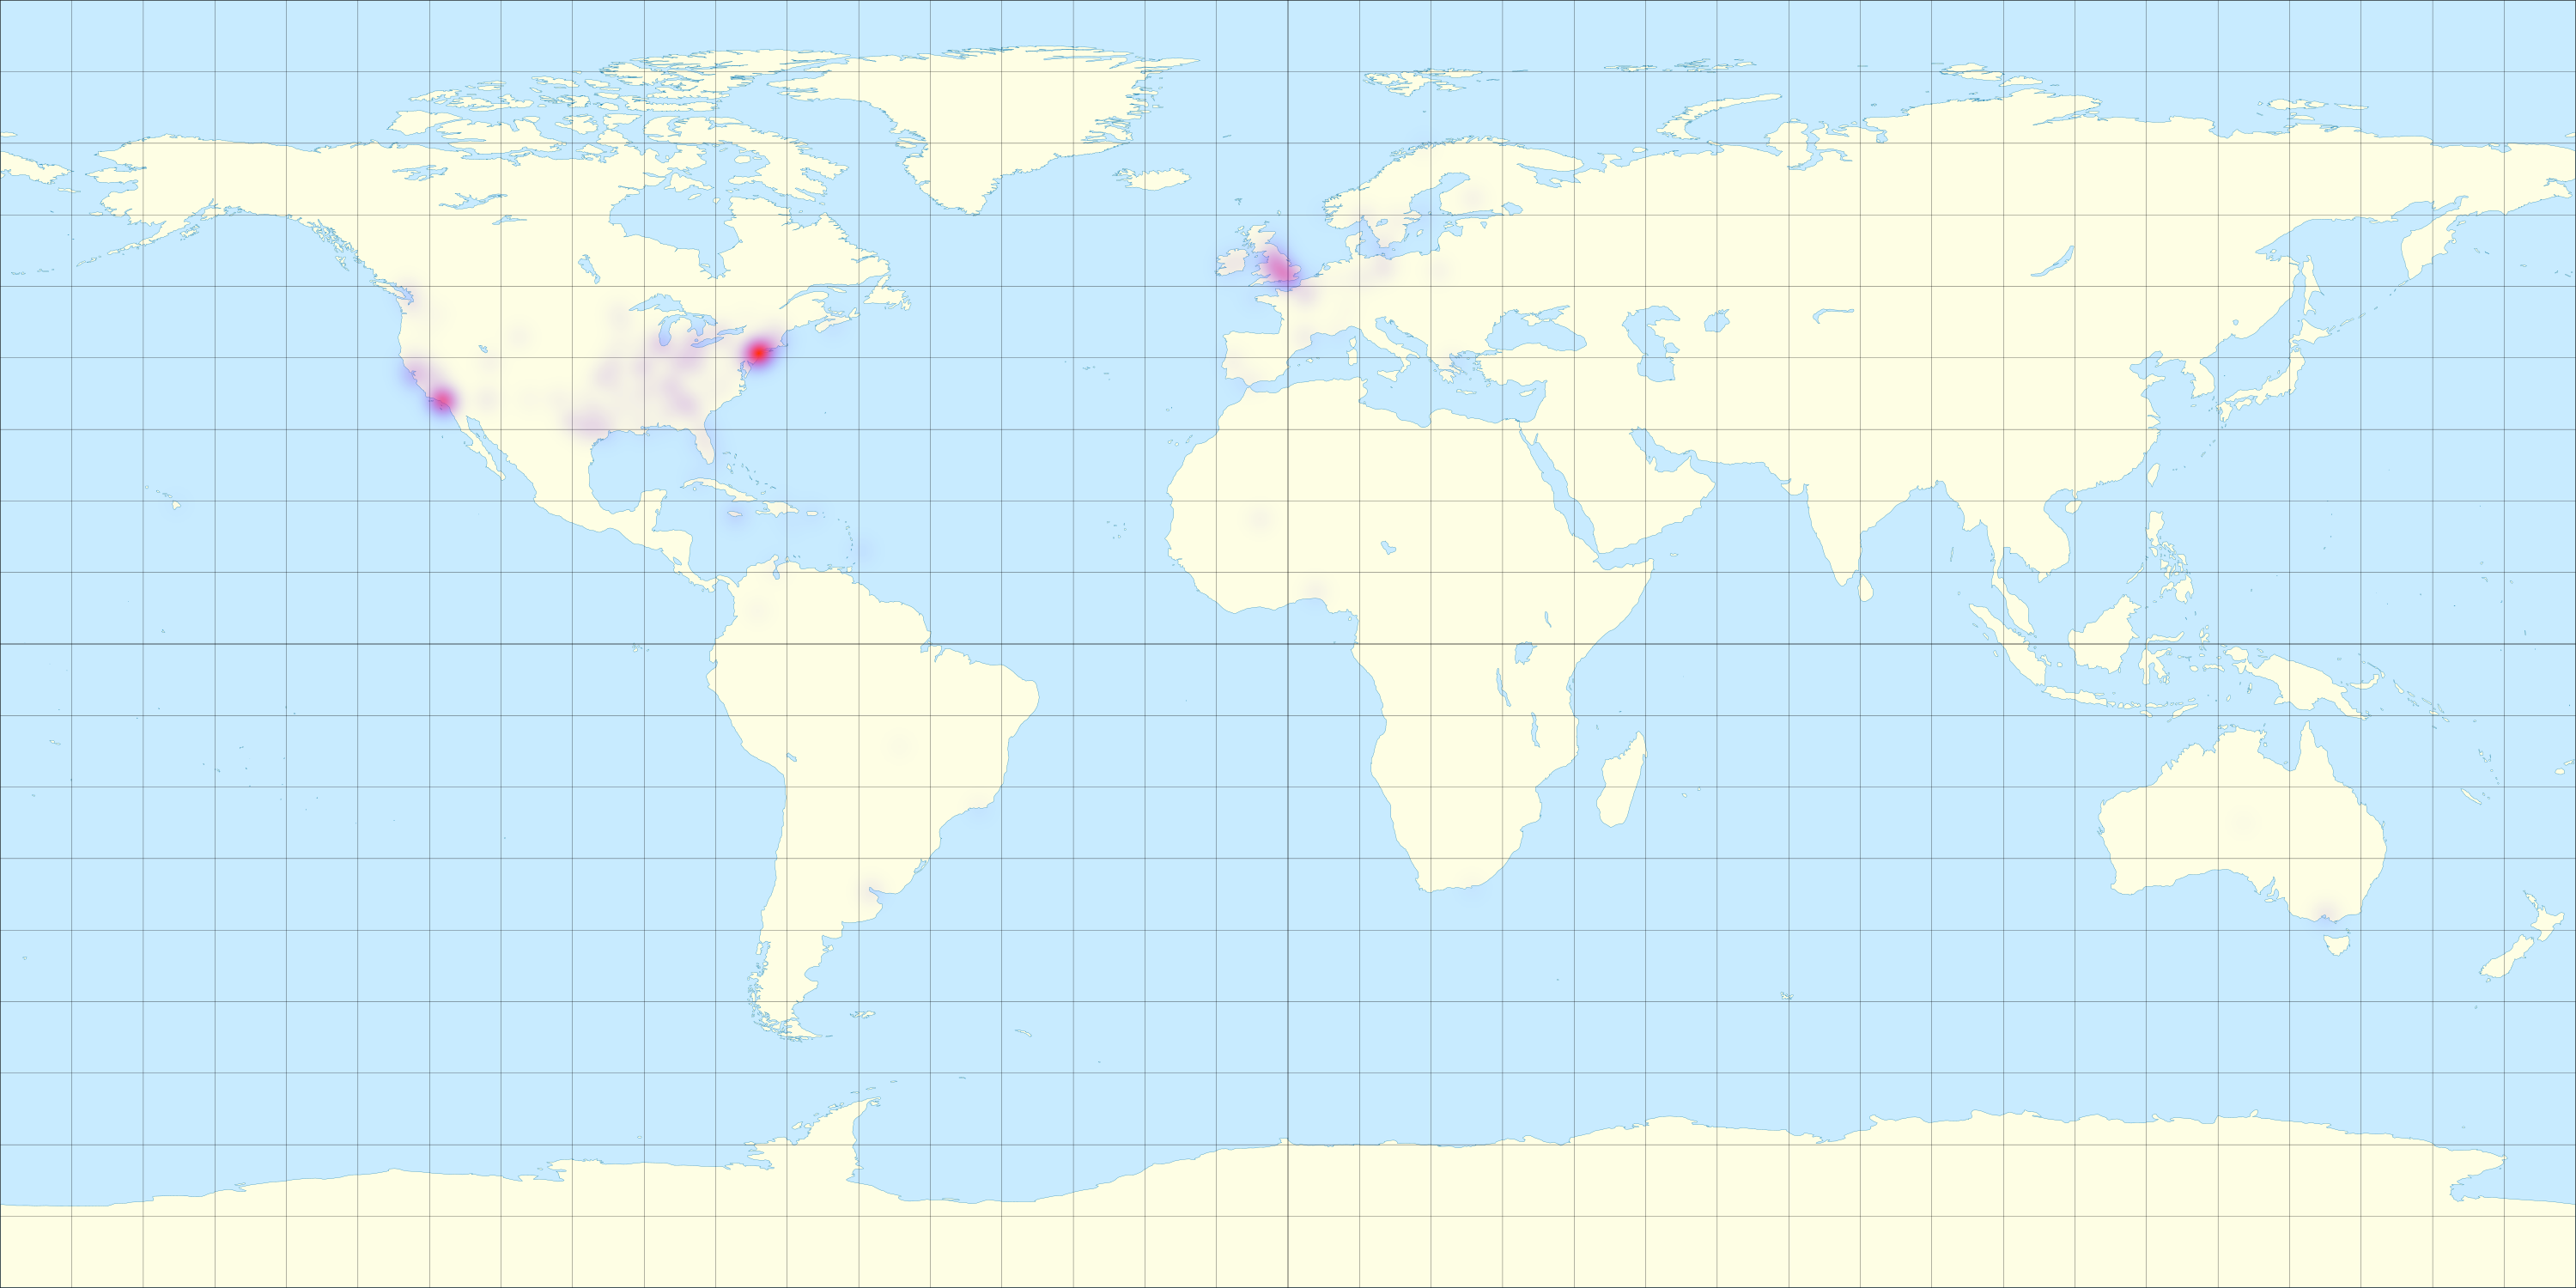
\includegraphics[width=\linewidth]{../../results/average-song-hotttnesss-by-artist-B}}
    \captionof{figure}[Artist's average song hotttnesss plotted on a map based on the song's artist's location.]{%
        Artist's average song hotttnesss plotted on a map based on the song's artist's location (if known).
        Adapted from \textcite{gaba2008tissot}.
    }
    \label{fig:average-song-hotttnesss-by-artist-b}
\end{minipage}

\subsection{Source code and raw data}

The source code and scripts for running 
this analysis as well as the unedited 
map-reduce outputs can be found publicly 
on the corresponding repository at 
\url{https://github.com/heinrichreimer/song-analysis}.
The repository provides installation scripts for Linux
and Gradle build tasks for each analysis task,
including some not mentioned in this thesis. 

%%%%%%%%%%%%%%%%%%%%%%%%%%%%%%%%%%%%%%%%%%%%%%%%%%%%%%%%%%%%%%%%%%%%%%%%%%%%%%%%%
%% Ende des Dokuments                                                          %%
%%%%%%%%%%%%%%%%%%%%%%%%%%%%%%%%%%%%%%%%%%%%%%%%%%%%%%%%%%%%%%%%%%%%%%%%%%%%%%%%%
\end{document}                                                                  %
